\documentclass{homework}
\usepackage[shortlabels]{enumitem}
\usepackage{listings}
\usepackage{xcolor}
\usepackage{amsmath}

\definecolor{codegreen}{rgb}{0,0.6,0}
\definecolor{codegray}{rgb}{0.5,0.5,0.5}
\definecolor{codepurple}{rgb}{0.58,0,0.82}
\definecolor{backcolour}{rgb}{0.95,0.95,0.92}

\lstdefinestyle{mystyle}{
    backgroundcolor=\color{backcolour},   
    commentstyle=\color{codegreen},
    keywordstyle=\color{magenta},
    numberstyle=\tiny\color{codegray},
    stringstyle=\color{codepurple},
    basicstyle=\ttfamily\footnotesize,
    breakatwhitespace=false,         
    breaklines=true,    captionpos=b,                    
    keepspaces=true, numbers=left,                    
    numbersep=5pt, showspaces=false,                
    showstringspaces=false, showtabs=false, tabsize=2}
\lstset{style=mystyle}


\usepackage{titling}
\renewcommand\maketitlehooka{\null\mbox{}\vfill}
\renewcommand\maketitlehookd{\vfill\null}

\makeatletter
% we use \prefix@<level> only if it is defined
\renewcommand{\@seccntformat}[1]{%
  \ifcsname prefix@#1\endcsname
    \csname prefix@#1\endcsname
  \else
    \csname the#1\endcsname\quad
  \fi}
% define \prefix@section
\newcommand\prefix@section{Problème \thesection }
\makeatother

\title{\textbf{STT 6615: Séries chronologiques}\\Devoir 1\\Automne 2024}
\author{\textbf{Christian L. Goueguel}}

\begin{document}

\begin{titlingpage}
\maketitle
\end{titlingpage}
%-----------------------------------------------------------------------------
\textbf{\Large{Problème 1.1}}

To compare the earthquake and explosion signals, plot the data displayed in \textbf{Figure 1.7} on the same graph using different colors or different line types and comment on the results. \\

\textit{\textbf{Solution:}}

Dans le graphique ci-dessous, nous avons superposé les signaux de l'explosion (en bleu) et du tremblement de terre (en rouge).

\begin{figure}[h]
    \centering
    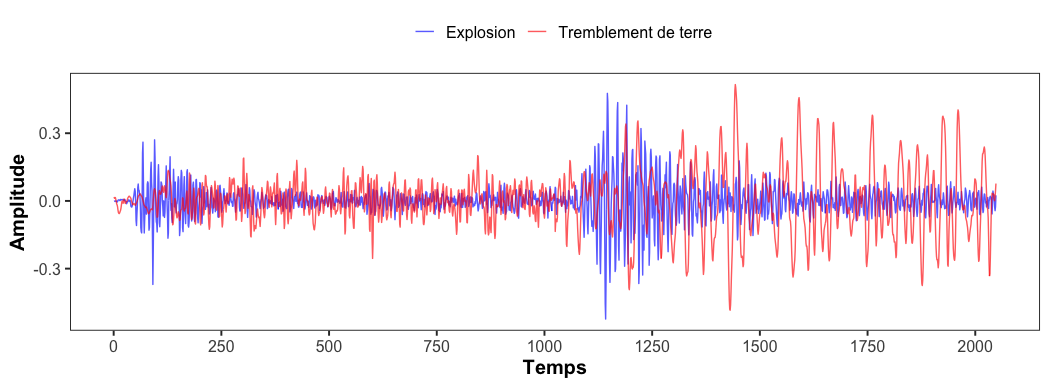
\includegraphics[width=1\linewidth]{figure1.1.png}
\end{figure}

On observe qu'avant $t=1000$, les deux signaux montrent des fluctuations de faible amplitude. Entre $t=1000$ et $t=1250$, l'explosion et le tremblement de terre semblent se produire simultanément. Les deux signaux commencent à fluctuer de manière significative. De plus, le signal de l'explosion semble avoir une durée de vie plus courte, tandis que le signal du tremblement de terre montre des fluctuations importantes sur une période plus longue après le début de l'événement.
%-----------------------------------------------------------------------------
\newpage
\textbf{\Large{Problème 1.2}}

Consider a signal-plus-noise model of the general form $x_t = s_t + w_t$, where $w_t$ is Gaussian white noise with $\sigma^2_w = 1$. Simulate and plot $n = 200$ observations from each of the following two models.
\begin{enumerate}[(a)]
    \item $x_t = s_t + w_t$, for $t = 1, \dots, 200$, where

$$s_t = \left\{
    \begin{array}{l l} 
        0, & t = 1, \dots, 100 \\ 
        10\exp\left(-\frac{(t - 100)}{20}\right)\cos(2\pi t / 4), & t = 101, \dots, 200
    \end{array}
  \right.$$
  \item $x_t = s_t + w_t$, for $t = 1, \dots, 200$, where

$$s_t = \left\{
    \begin{array}{l l} 
        0, & t = 1, \dots, 100 \\ 
        10\exp\left(-\frac{(t - 100)}{200}\right)\cos(2\pi t / 4), & t = 101, \dots, 200
    \end{array}
  \right.$$

   \item Compare the general appearance of the series (a) and (b) with the earthquake series and the explosion series shown in Figure 1.7. In addition, plot (or sketch) and compare the signal modulators (a) $\exp{(-t/20)}$ and (b) $\exp{(-t/200)}$, for $t = 1,2,\dots,100$.
\end{enumerate}

\vspace{1cm}

\textit{\textbf{Solution:}}\\
Supposons le modèle signal plus bruit suivant :
$$x_t = s_t + w_t, \quad w_t \sim \mathcal{N}(0, 1)$$


\textbf{(a)} On obtient le graphique ci-dessous, lorsque $s_t$ est définit par
    $$s_t = \left\{
    \begin{array}{l l} 
        0, & t = 1, \dots, 100 \\ 
        10\exp\left(-\frac{(t - 100)}{20}\right)\cos(2\pi t / 4), & t = 101, \dots, 200
    \end{array}
  \right.$$
\begin{figure}[h]
    \centering
    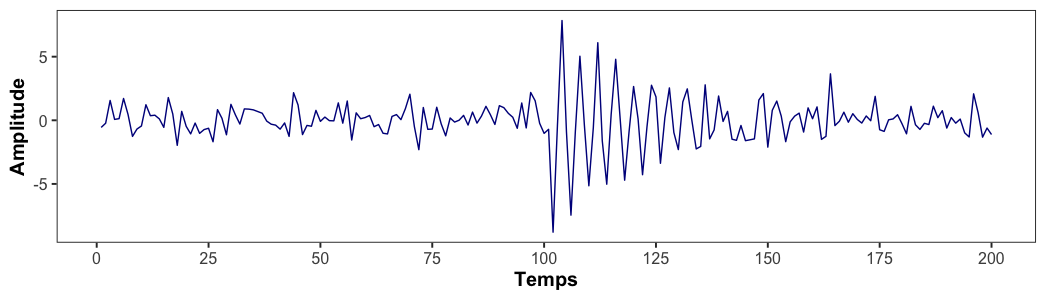
\includegraphics[width=1\linewidth]{figure1.2a.png}
\end{figure}

    \newpage
    
\textbf{(b)} On obtient le graphique ci-dessous, lorsque $s_t$ est définit par
    $$s_t = \left\{
    \begin{array}{l l} 
        0, & t = 1, \dots, 100 \\ 
        10\exp\left(-\frac{(t - 100)}{200}\right)\cos(2\pi t / 4), & t = 101, \dots, 200
    \end{array}
  \right.$$
\begin{figure}[h]
    \centering
    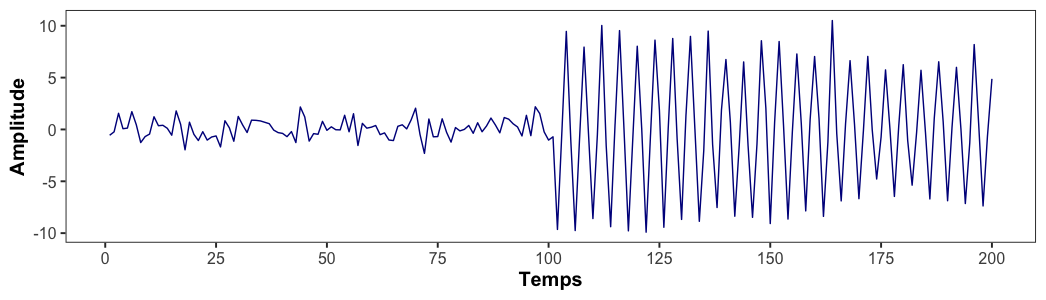
\includegraphics[width=1\linewidth]{figure1.2b.png}
\end{figure}
    
\textbf{(c)} En comparant les séries (a) et (b) aux sismogrammes présentés dans le \textbf{Problème 1.1}, on peut observer des similarités :

\begin{enumerate}
    \item La série (a) présente des caractéristiques proches de celles du sismogramme d'explosions. Elle se distingue par:
    \begin{enumerate}
        \item[\textbullet] une augmentaion rapide et abrupte de l'amplitude du signal
        \item[\textbullet] une décroissance relativement rapide du signal
        \item[\textbullet] des oscillations plus régulières et de plus haute fréquence
    \end{enumerate} 
     
    \item En revanche, la série (b) montre une ressemblance significative avec le sismogramme de tremblements de terre. Ses traits distinctifs incluent:
    \begin{enumerate}
        \item[\textbullet] une augmentation plus rapide de l'amplitude
        \item[\textbullet] une décroissance plus lente et prolongée du signal
        \item[\textbullet] des oscillations plus irrégulières et de plus basse fréquence
    \end{enumerate} 
\end{enumerate}

Procédons à la visualisation des modulateurs des signaux (a) $\exp(-t / 20)$ et (b) $\exp(-t / 200)$, pour $t = 1, \dots, 100$, que nous pouvons réécrire sous forme: $\exp(-t\lambda)$, avec $\lambda$ la constante de décroissance, égale à 1/20 et 1/200, pour les modulateurs (a) et (b), respectivement.

À partir de la figure ci-dessous, on observe que l'intensité du modulateur de signal (a) décroît beaucoup plus rapidement que celle du modulateur de signal (b). La différence d'un ordre de grandeur entre la constante de temps ($\tau = 1/\lambda$) du modulateur (a) $\tau = 20$ et (b) $\tau = 200$ explique les comportements observés. Ce qui implique qu'une petite valeur de $\tau$ (cas a) indique une dissipation d'énergie plus rapide, typique des phénomènes explosifs. Tandit qu'une plus grande valeur de $\tau$ (cas b) suggère une libération d'énergie plus lente, caractéristique des tremblements de terre.

\begin{figure}
    \centering
    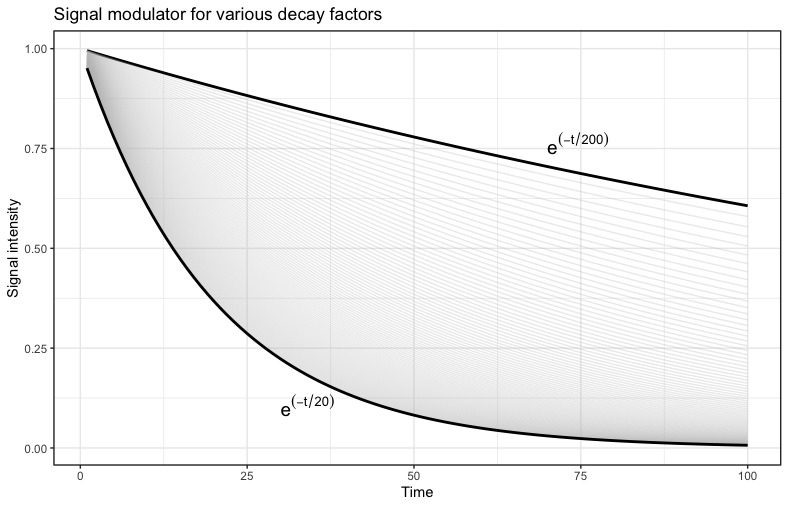
\includegraphics[width=1\linewidth]{figure1.2c.png}
\end{figure}
\newpage
\empty
\section*{}
%-----------------------------------------------------------------------------
\newpage
\textbf{\Large{Problème 1.3}}

\begin{enumerate}[(a)]
    \item Generate $n = 100$ observations from the autoregression $$x_t = -0.9x_{t-2} + w_t$$ with $\sigma_w = 1$, using the method described in Example 1.10. Next, apply the moving average filter $$\nu_t = (x_t + x_{t-1} + x_{t-2} + x_{t-3})/4$$ to $x_t$ , the data you generated. Now plot $x_t$ as a line and superimpose $\nu_t$ as a dashed line. Comment on the behavior of $x_t$ and how applying the moving average filter changes that behavior.
    \item Repeat (a) but with $$x_t = \cos(2 \pi t/4)$$
    \item Repeat (b) but with added $\mathcal{N}(0, 1)$ noise, $$x_t = \cos(2 \pi t/4) + w_t$$
    \item Compare and contrast (a)–(c); i.e., how does the moving average change each series?
\end{enumerate}

\textit{\textbf{Solution:}}\\
\textbf{(a)} Le graphique ci-dessous illustre la superimposition des séries $x_t$ et $\nu_t$. 

\begin{figure}[h]
    \centering
    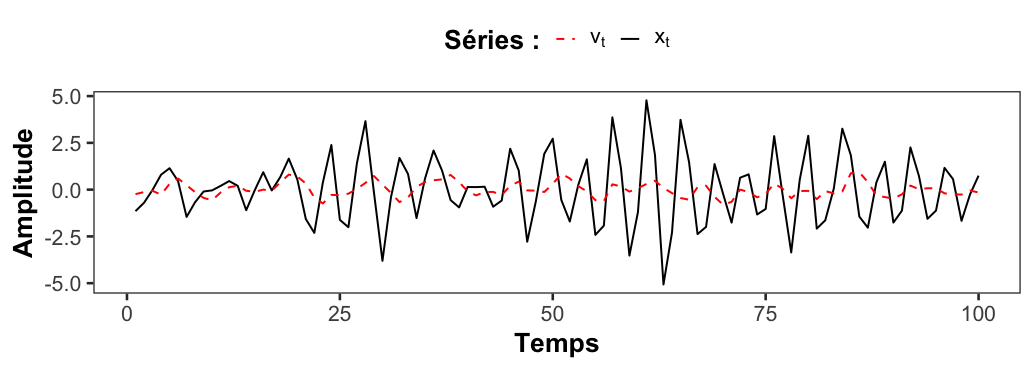
\includegraphics[width=1\linewidth]{figure1.3a.png}
\end{figure}

On observe que l'amplitude de la série $x_t$ oscille fortement, présentant des fluctuations importantes et rapides. Ces oscillations sont dûe à la nature stochastique du processus autorégressif de second ordre, défini par l'équation $x_t = -0.9x_{t-2} + w_t$. En appliquant le filtre de moyenne mobile, $\nu_t$, celui-ci atténue les fluctuations observées dans $x_t$. En sommes, le filtre de moyenne mobile permet de réduire efficacement le bruit de la série $x_t$.

\textbf{(b)} Lorsqu'on considère le modèle $x_t = \cos(2 \pi t/4)$, on obtient le graphique suivant:











%-----------------------------------------------------------------------------
\newpage
\textbf{\Large{Problème 1.6}}

Consider the time series $$x_t = \beta_1 + \beta_2 t + w_t$$
where $\beta_1$ and $\beta_2$ are known constants and $w_t$ is a white noise process with variance $\sigma^2_w$.

\begin{enumerate}[(a)]
    \item Determine whether $x_t$ is stationary.
    \item Show that the process $y_t = x_t - x_{t-1}$ is stationary.
    \item Show that the mean of the moving average
    $$\nu_t = \frac{1}{2q + 1} \sum_{j=-q}^{q}x_{t-j}$$
    is $\beta_1 + \beta_2 t$, and give a simplified expression for the autocovariance function.
\end{enumerate}

\textit{\textbf{Solution:}}\\
\textbf{(a)} Par définition, la série $x_t$ est dite stationnaire, si elle vérifie les deux critères suivants :
\begin{enumerate}[(i)]
    \item la fonction moyenne $\mu_{x_t}$ ne dépend pas de $t$
    \item la fonction d’autocovariance $\gamma_{x_t}$ dépend uniquement du décalage temporel $h$. 
\end{enumerate}

Par ailleurs, rappelons que :
\begin{itemize}
    \item[\textbullet] $\mathbb{E}[w_t] = 0$
    \item[\textbullet] $\mathbb{E}[w_t^2] = \sigma^2_w$
    \item[\textbullet] $\mathbb{E}[w_tw_s] = 0$ pour $t \neq s$ 
\end{itemize}

Commençons par calculer la moyenne :
\begin{flalign*}
\mu_{x_t} &= \mathbb{E}[x_t]\\
          &= \mathbb{E}[\beta_1 + \beta_2 t + w_t]\\
          &= \mathbb{E}[\beta_1] + \mathbb{E}[\beta_2 t] + \mathbb{E}[w_t]\\
          &= \beta_1 + \beta_2 \mathbb{E}[t] \\
          &= \beta_1 + \beta_2 t
\end{flalign*}
Maintenant, calculons l'autocovariance :
\begin{flalign*}
\gamma_{x_t}(h) &= \text{cov}(x_{t+h}, x_t)\\
                &= \mathbb{E}[(x_{t+h} - \mu_{x_{t+h}})(x_t - \mu_{x_t})] \\
                &= \mathbb{E}[(\beta_1 + \beta_2(t+h) + w_{t+h} - (\beta_1 + \beta_2(t+h)))(\beta_1 + \beta_2t + w_t - (\beta_1 + \beta_2t))] \\
                &= \mathbb{E}[w_{t+h}w_t]
\end{flalign*}
À ce stade, nous devons considérer les deux cas suivants :
\begin{itemize}
    \item[\textbullet] $h = 0 \Rightarrow \gamma_{x_t}(0) = \mathbb{E}[w_t^2] = \text{Var}(w_t) = \sigma^2_w$
    \item[\textbullet] $h \neq 0 \Rightarrow \gamma_{x_t}(h) = \mathbb{E}[w_{t+h}w_t] = 0$
\end{itemize}
Donc, la fonction d'autocovariance devient :
$
\gamma_{x_t}(h) = \left\{
                    \begin{array}{r c l}
                        \sigma^2_w &\text{si}& h = 0 \\
                        0          &\text{si}& h \neq 0
\end{array}
               \right.
$               

On voit que la fonction d'autocovariance ne dépend que de $h$, ce qui est une propriété des processus stationnaires. Cependant, comme la fonction moyenne $\mu_{x_t} = \beta_1 + \beta_2 t$ dépend de $t$, ce qui est une condition suffisante pour conlure que la série $x_t$ n'est pas stationnaire.

\textbf{(b)} Considérons la série suivante :
\begin{flalign*}
y_t &= x_t - x_{t - 1} \\
    &= [\beta_1 + \beta_2 t + w_t] - [\beta_1 + \beta_2 (t-1) + w_{t-1}] \\
    &= \beta_2 + w_t - w_{t-1}
\end{flalign*}
Pour démontrer que cette série est stationnaire, nous allons appliquer le même raisonnement que celui utilisée précédemment dans la partie (a).

La moyenne de la série $y_t$ est donnée par :
\begin{flalign*}
\mu_{y_t} &= \mathbb{E}[y_t]\\
          &= \mathbb{E}[\beta_2 + w_t - w_{t-1}]\\
          &= \mathbb{E}[\beta_2] + \mathbb{E}[w_t] - \mathbb{E}[w_{t-1}] \\
          &= \beta_2
\end{flalign*}

Tandis que sa finction d'autocovariance est donnée par :
\begin{align*}
\gamma_{y_t}(h) &= \text{cov}(y_{t+h}, y_t) \\
          &= \mathbb{E}[(y_{t+h} - \mathbb{E}[y_{t+h}])(y_t - \mathbb{E}[y_t])] \\
          &= \mathbb{E}[y_{t+h} y_t - y_{t+h} \mathbb{E}[y_t] - y_t \mathbb{E}[y_{t+h}] + \mathbb{E}[y_{t+h}] \mathbb{E}[y_{t}]] \\ 
          & = \mathbb{E}[y_{t+h} y_t - \beta_2 y_{t+h} - \beta_2 y_t + \beta^2_2] \\
          &= \mathbb{E}[(\beta_2 + w_{t+h} - w_{t+h-1})(\beta_2 + w_t - w_{t-1}) - \beta_2(\beta_2 + w_{t+h} - w_{t+h-1}) - \beta_2(\beta_2 + w_t - w_{t-1}) + \beta_2^2] \\
          &= \mathbb{E}[w_{t+h}w_t - w_{t+h}w_{t-1} - w_{t+h-1}w_t + w_{t+h-1}w_{t-1}] \\
          &= \mathbb{E}[w_{t+h}w_t] - \mathbb{E}[w_{t+h}w_{t-1}] - \mathbb{E}[w_{t+h-1}w_t] + \mathbb{E}[w_{t+h-1}w_{t-1}]
\end{align*}
Considérons les cas suivants :
\begin{itemize}
    \item[\textbullet] $h = 0 \Rightarrow \gamma_{y_t}(0) = \mathbb{E}[w_t^2] + \mathbb{E}[w_{t-1}^2]  = 2\sigma^2_w$
    \item[\textbullet] $h = 1 \Rightarrow \gamma_{y_t}(1) = -\mathbb{E}[w_t^2] = -\sigma_w^2$
    \item[\textbullet] $h = -1 \Rightarrow \gamma_{y_t}(-1) = -\mathbb{E}[w_{t-1}^2] = -\sigma_w^2$
    \item[\textbullet] $\vert h \vert \ > 1 \Rightarrow \gamma_{y_t} (\vert h \vert) = 0$
\end{itemize}
Ainsi, la fonction d'autocovariance peut être exprimée sous la forme suivante :
\begin{align*}
\gamma_{y_t}(h) &= \left\{
                \begin{array}{r c l}
                    2\sigma_w^2 &\text{si}& h = 0\\
                    -\sigma_w^2 &\text{si}& \vert h \vert = 1\\
                    0           &\text{si}& \vert h \vert > 1
                \end{array}
             \right.
\end{align*}

Par conséquent, nous pouvons conclure que la série $y_t$ est stationnaire, puisque nous avons montré que sa moyenne est indépendante de $t$ et que sa fonction d'autocovariance dépent uniquement de $h$.

\textbf{(c)} Pour démontrer que la moyenne de la moyenne mobile est : $\mu_{\nu_t} = \beta_1 + \beta_2t$ \\
On écrit :
\begin{align*}
\mu_{\nu_t} &= \mathbb{E}(\nu_t) \\
             &= \mathbb{E}\left(\frac{1}{2q + 1}\sum_{j=-q}^{q}x_{t-j}\right) \\
             &= \frac{1}{2q + 1}\sum_{j=-q}^{q}\mathbb{E}[x_{t-j}] \\
             &= \frac{1}{2q + 1}\sum_{j=-q}^{q}\mathbb{E}[\beta_1 + \beta_2(t-j) + w_{t-j}] \\
             &= \frac{1}{2q + 1}\sum_{j=-q}^{q}(\mathbb{E}[\beta_1] + \mathbb{E}[\beta_2 t] - \mathbb{E}[\beta_2 j] + \mathbb{E}[w_{t-j}]) \\
             &= \frac{1}{2q + 1}\sum_{j=-q}^{q}(\beta_1 + \beta_2 t - \beta_2 j) \\
             &= \frac{\beta_1}{2q + 1} + \frac{\beta_2t}{2q + 1} - \frac{\beta_2}{2q + 1}\sum_{j=-q}^{q}j \\
             &= \frac{1}{2q + 1}\left((2q+1)\beta_1 + (2q+1)\beta_2 t - \beta_2\sum_{j=-q}^{q}j\right) \\
             &= \beta_1 + \beta_2t - \frac{\beta_2}{2q+1}\sum_{j=-q}^{q}j
\end{align*}
Or, $\sum_{j=-q}^{q}j = 0$ car la somme est symétrique autour de zéro.\\
Par conséquent, on obtient :
\begin{align*}
\mu_{\nu_t} &= \beta_1 + \beta_2t \quad  \blacksquare
\end{align*}

La fonction d'autocovariance est donnée par :
\begin{align*}
\gamma_{\nu_t}(h) &= \text{Cov}(\nu_{t+h}, \nu_t) \\
          &= \text{Cov}\left( \frac{1}{2q + 1}\sum_{j=-q}^{q}x_{t-j+h}, \frac{1}{2q + 1}\sum_{j=-q}^{q}x_{t-j} \right) \\
          &= \left( \frac{1}{2q + 1} \right)^2 \text{Cov} \left( \sum_{j=-q}^{q}w_{t-j+h}, \sum_{j=-q}^{q}w_{t-j} \right) \\
          &= \left( \frac{1}{2q + 1} \right)^2 \mathbb{E}\left[ \left( \sum_{j=-q}^{q}w_{t-j+h} - \mathbb{E} \left[ \sum_{j=-q}^{q}w_{t-j+h} \right] \right) \left( \sum_{j=-q}^{q}w_{t-j} - \mathbb{E}\left[ \sum_{j=-q}^{q}w_{t-j} \right] \right) \right] \\
          &= \left( \frac{1}{2q + 1} \right)^2 \sum_{j=-q}^q \mathbb{E}\left[ \left( w_{t-j+h} - \mathbb{E}[w_{t-j+h}] \right) \left( w_{t-j} - \mathbb{E}[w_{t-j}] \right) \right] \\
          &= \left( \frac{1}{2q + 1} \right)^2 \sum_{j=-q}^q \mathbb{E}\left[ w_{t-j+h}w_{t-j} \right]
\end{align*}
Considérons les cas suivants :
\begin{itemize}
    \item[\textbullet] $h = 0 \Rightarrow \gamma_{\nu_t}(0) = \left( \frac{1}{2q + 1} \right)^2 \sum_{j=-q}^q \mathbb{E}\left[ w_{t-j}^2 \right] = \left( \frac{\sigma_w}{2q + 1} \right)^2$
    \item[\textbullet] $h \neq 0 \Rightarrow \gamma_{\nu_t}(h) = \left( \frac{1}{2q + 1} \right)^2 \mathbb{E}\left[ w_{t-j+h}w_{t-j} \right] = 0$
\end{itemize}
Par conséquent, 
$
\gamma_{\nu_t}(h) = 
\left\{
\begin{array}{c c l}
    \left( \frac{\sigma_w}{2q + 1} \right)^2  & \text{si} & h = 0\\
                 0                            & \text{si} & h \neq 0
\end{array}
\right.
$
%-----------------------------------------------------------------------------
\newpage
\textbf{\Large{Problème 1.7}}

For a moving average process of the form
$$x_t = w_{t-1} + 2w_t + w_{t+1}$$
where $w_t$ are independent with zero means and variance $\sigma^2_w$, determine the autocovariance and autocorrelation functions as a function of lag $h = s-t$ and plot the ACF as a function of $h$.

\textit{\textbf{Solution:}}\\
Considérons la moyenne mobile suivante : 
$$x_t = w_{t-1} + 2w_t + w_{t+1} \quad w_t \sim \mathcal{N}(0, \sigma^2_w)$$
La fonction d'autocovariance est donnée par :
\begin{align*}
\gamma_{x_t}(h) &= \text{Cov}(x_{t+h}, x_t) \\
          &= \mathbb{E}[(x_{t+h} - \mathbb{E}[x_{t+h}])(x_{t} - \mathbb{E}[x_{t}])] \\
          &= \mathbb{E}[(w_{t-1+h} + 2w_{t+h} - w_{t+1+h})(w_{t-1} + 2w_{t} - w_{t+1})] \\
          &= \mathbb{E}[w_{t-1+h}w_{t-1} + 2w_{t-1+h}w_t - w_{t-1+h}w_{t+1} + 2w_{t+h}w_{t-1} + 4w_{t+h}w_t - 2w_{t+h}w_{t+1} - w_{t+1+h}w_{t-1} \\
          &- 2w_{t+1+h}w_t + w_{t+1+h}w_{t+1}]
\end{align*}

Considérons les cas suivants :
\begin{itemize}
    \item[\textbullet] $h = 0 \Rightarrow \gamma_{x_t}(0) = \mathbb{E}[w_{t-1}^2 + 4w_t^2 + w_{t+1}^2] = 6\sigma_w^2$
    \item[\textbullet] $h = 1 \Rightarrow \gamma_{x_t}(1) = \mathbb{E}[2w_t^2 - 2w_{t+1}^2] = 2\mathbb{E}[(w_t - w_{t+1})^2] = 2\sigma_w^2 $
    \item[\textbullet] $h = -1 \Rightarrow \gamma_{x_t}(-1) = \mathbb{E}[2w_{t-1}^2 - 2w_{t+1}^2] = 2\mathbb{E}[(w_{t-1}-w_{t+1})^2] = 2\sigma_w^2$
    \item[\textbullet] $h = 2 \Rightarrow \gamma_{x_t}(2) =$
    \item[\textbullet] $h = -2 \Rightarrow \gamma_{x_t}(-2) =$
\end{itemize}
On obtient :
$$
\gamma_{x_t}(h) = 
\left\{ 
\begin{array}{c c l}
6\sigma_w^2 & \text{si} & s=t\\
4\sigma_w^2 & \text{si} & \vert s-t \vert = 1\\
\sigma_w^2  & \text{si} & \vert s-t \vert = 2\\
0           & \text{si} & \vert s-t \vert > 2\\
\end{array}
\right.
$$

La fonction d'autocorrélation ACF est donnée par :
\begin{align*}
\rho_{x_t}(h) &= \frac{\gamma_{x_t}(t+h,t)}{\sqrt{\gamma_{x_t}(t+h,t+h)\gamma_{x_t}(t,t)}} \\
        &= \frac{\gamma_{x_t}(h)}{\gamma_{x_t}(0)} \\
        &= \frac{1}{6\sigma_w^2} \left\{ 
\begin{array}{c c l}
6\sigma_w^2 & \text{si} & s=t\\
4\sigma_w^2 & \text{si} & \vert s-t \vert = 1\\
\sigma_w^2  & \text{si} & \vert s-t \vert = 2\\
0           & \text{si} & \vert s-t \vert > 2\\
\end{array}
\right.\\
        &= \left\{
             \begin{array}{c c l}
               1   & \text{si} & s=t\\
               2/3 & \text{si} & \vert s-t \vert = 1\\
               1/6 & \text{si} & \vert s-t \vert = 2\\
               0   & \text{si} & \vert s-t \vert > 2\\
             \end{array}
           \right.
\end{align*}

Le graphique ci-dessous illustre la fonction d'autocorrélation en fonction de $h$ : 
\begin{figure}[h]
    \centering
    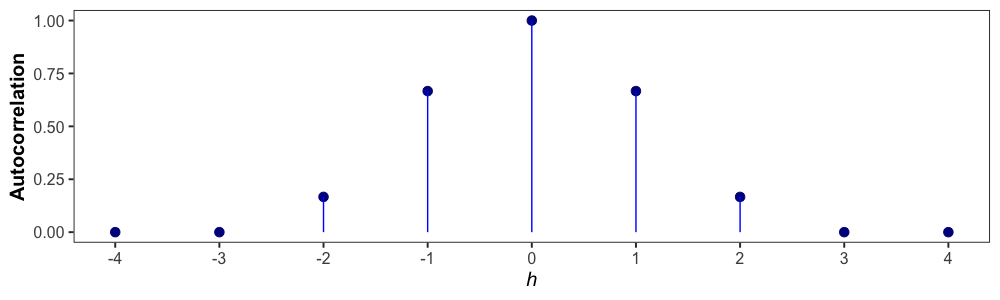
\includegraphics[width=1\linewidth]{figure1.7.png}
\end{figure}
\newpage
\empty
\section*{}
%-----------------------------------------------------------------------------
\newpage
\textbf{\Large{Problème 1.13}}

Consider the two series
$$x_t = w_t$$
$$y_t = w_t - \theta w_{t-1} + u_t$$
where $w_t$ and $u_t$ are independent white noise series with variances $\sigma^2_w$ and $\sigma^2_u$, respectively, and $\theta$ is an unspecified constant.
\begin{enumerate}[(a)]
    \item Express the ACF, $\rho_y(h)$, for $h = 0, \pm1, \pm2,...$ of the series $y_t$ as a function of $\sigma^2_w$, $\sigma^2_u$, $\theta$.
    \item Determine the CCF, $\rho_{xy}(h)$ relating $x_t$ and $y_t$.
    \item Show that $x_t$ and $y_t$ are jointly stationary.\\
\end{enumerate}
\textit{\textbf{Solution:}}\\
\textbf{(a)} La fonction d'autocorrélation, ACF, est définit par :
$$
\rho_y(h) = \frac{\gamma_y(h)}{\gamma_y(0)}
$$
Avec, $\gamma_y(h)$ la fonction d'autocovariance, ACVF, donnée par : 
$$
\gamma_y(h) = \text{cov}(y_{t+h}, y_t) \\
            = \text{cov}(w_{t+h} - \theta w_{t-1+h} + u_{t+h}, w_t - \theta w_{t-1} + u_t) \\
            = \left\{
                \begin{array}{c l l}
                    (1 + \theta^2)\sigma_w^2 + \sigma_u^2 &\text{si}& h = 0\\
                    -\theta\sigma_w^2 &\text{si}& |h| = 1 \\
                    0 &\text{sinon}&
                \end{array}
               \right.
$$
Ce qui donne :
$$
\rho_y(h) = \left\{
                \begin{array}{c l l}
                    1 &\text{si}& h = 0\\
                    -\frac{\theta\sigma_w^2}{(1 + \theta^2)\sigma_w^2 + \sigma_u^2} &\text{si}& |h| = 1 \\
                    0 &\text{sinon}&
                \end{array}
               \right.
$$

\textbf{(b)} La fonction de corrélation croisée, CCF, est définit par :
\begin{align*}
\rho_{xy}(h) &= \frac{\gamma_{xy}(h)}{\sqrt{\gamma_x(0)\gamma_y(0)}} 
\end{align*}
avec,
$$\gamma_x(0) = \text{cov}(w_t,w_t) = \sigma_w^2, \quad \gamma_y(0) = (1 + \theta^2)\sigma_w^2 + \sigma_u^2$$
et la fonction de covariance croisée, $\gamma_{xy}(h)$, donnée par :
$$
\gamma_{xy}(h) = \text{cov}(x_{t+h}, y_t) \\
               = \text{cov}(w_{t+h}, w_t - \theta w_{t-1} + u_t) \\
               = \left\{
                    \begin{array}{c l l}
                        \sigma_w^2 &\text{si}& h = 0\\
                        -\theta\sigma_w^2 &\text{si}& h = -1 \\
                        0 &\text{sinon}&
                    \end{array}
                \right.
$$
On obtient finalement :
\begin{align*}
\rho_{xy}(h) &= \frac{1}{\sqrt{\sigma_w^2((1 + \theta^2)\sigma_w^2 + \sigma_u^2)}}\left\{
                    \begin{array}{c l l}
                        \sigma_w^2 &\text{si}& h = 0\\
                        -\theta\sigma_w^2 &\text{si}& h = -1 \\
                        0 &\text{sinon}&
                    \end{array}
                \right.
\end{align*}

\textbf{(c)} Par définition, les séries $x_t$ et $y_t$ sont dites conjointement stationnaires si :
\begin{enumerate}[(i)]
    \item $x_t$ et $y_t$ sont individuellement stationaires,
    \item la fonction de covariance croisée, $\gamma_{xy}$, ne dépend que du décalage temporel $h$.
\end{enumerate}
Or, en nous référant aux résultats obtenus précédemment dans la partie \textbf{(b)}, nous avons démontré la condition (ii) que $\gamma_{xy}$ ne dépend effectivement que de $h$. 

Il reste à vérifier la condition (i), que nous formulons ainsi :
La moyenne des séries $x_t$ et $y_t$ est nulle car $x_t$ et $y_t$ sont définit comme des bruits blanc. De plus, comme montré dans la partie \textbf{(a)}, la fonction d'autocovariance des séries $x_t$ et $y_t$ dépend uniquement de $h$.

Par conséquent, nous pouvons conclure que les séries $x_t$ et $y_t$ sont conjointement stationnaires.
%-----------------------------------------------------------------------------
\newpage
\textbf{\Large{Problème 1.20}}

\begin{enumerate}[(a)]
    \item Simulate a series of $n = 500$ Gaussian white noise observations as in \textbf{Example 1.8} and compute the sample ACF, $\hat{\rho}(h)$, to lag 20. Compare the sample ACF you obtain to the actual ACF, $\rho(h)$. [Recall Example 1.19.]
    \item Repeat part (a) using only $n = 50$. How does changing $n$ affect the results?\\
\end{enumerate}

\textit{\textbf{Solution:}}\\
\textbf{(a)} La première figure ci-dessous illustre une simulation du bruit blanc gaussien $ w_t \sim \mathcal{N}(0,1)$. Elle montre l'évolution temporelle d'une série de 500 observations. Tandis que la seconde figure montre l'estimation de la fonction d'autocorrélation (ACF), $\hat{\rho}(h)$, de la série simulée avec un décalage maximum $h_{max}=20$.  
\begin{figure}[h]
    \centering
    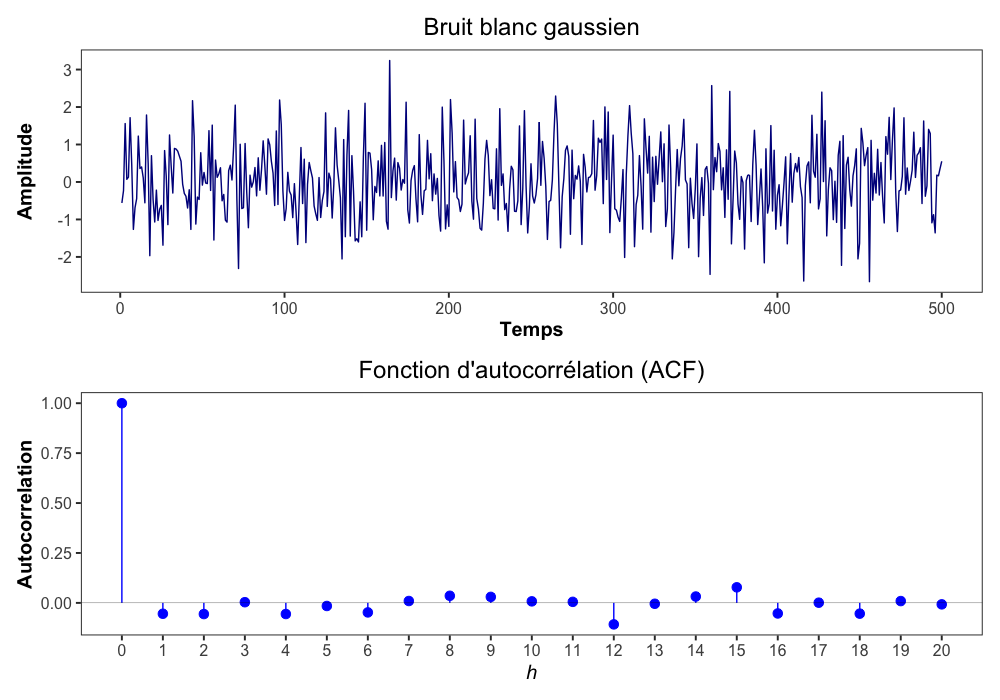
\includegraphics[width=1\linewidth]{figure1.20.png}
\end{figure}

En comparant $\hat{\rho}(h)$ à sa valeur réelle $\rho(h)$, on observe que les deux séries sont égales à 1 pour $h = 0$. En revanche, pour $h \neq 0$, $\rho(h) = 0$, tandis que $\hat{\rho}(h)$ semble converger vers 0.
\newpage
\textbf{(b)} Pour 50 observations, les graphiques obtenus sont les suivants :


\begin{figure}[h]
    \centering
    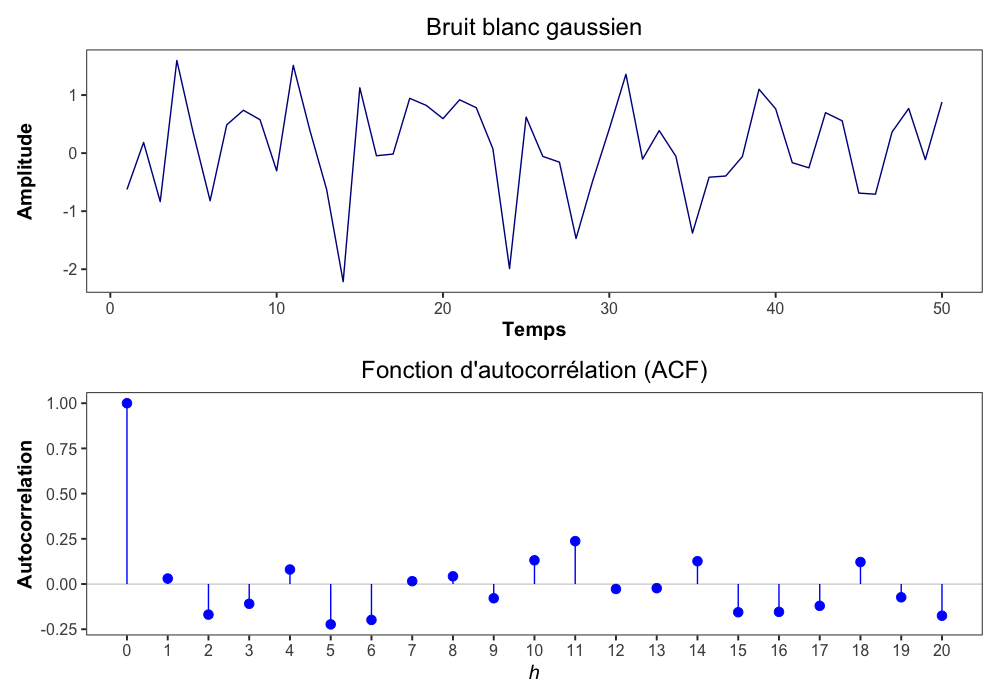
\includegraphics[width=1\linewidth]{figure1.20b.png}
\end{figure}

On observe que le nombre d'observations, $n$, influence significativement la convergence de la série $\hat{\rho}(h)$ vers 0 pour $h \neq 0$. En effet, lorsque $n = 500$, $\hat{\rho}(h)$ converge bien plus rapidement vers 0 qu'avec $n = 50$. 

%-----------------------------------------------------------------------------
\newpage
\textbf{\Large{Problème 1.25}}

A real-valued function $g(t)$, defined on the integers, is non-negative definite if and only if
$$
\sum_{i=1}^{n}\sum_{j=1}^{n}a_ig(t_i - t_j)a_j \geq 0
$$
for all positive integers $n$ and for all vectors $a = (a_1,a_2,...,a_n)^\top$ and $t = (t_1,t_2,...,t_n)^\top$. For the matrix $G = \{g(t_i - t_j); i,j = 1,2,...,n\}$, this implies that $a^\top Ga$ $\geq 0$ for all vectors $a$. It is called positive definite if we can replace '$\geq$' with '$>$' for all $a \neq 0$, the zero vector.
\begin{enumerate}[(a)]
    \item Prove that $\gamma(h)$, the autocovariance function of a stationary process, is a non-negative definite function.
    \item Verify that the sample autocovariance $\hat{\gamma}(h)$ is a non-negative definite function.\\
\end{enumerate}

\textit{\textbf{Solution:}}\\
\textbf{(a)} Démontrons que $\gamma(h)$, la fonction d'autocovariance d'un processus stationnaire, est une fonction non-négative définie.

Pour un processus stationnaire $\{x_t\}$, la fonction d'autocovariance est définie comme :
\[ \gamma(h) = \text{cov}(x_{t+h},x_t) = \mathbb{E}[(x_t - \mu)(x_{t+h} - \mu)] \]

Considérons une série $\{z_t\}$ la combinaison linéaire de $\{x_t\}$ telle que : 
$ z_t = \sum_{i=1}^n a_i (x_{t_i} - \mu) $

La variance de $z_t$ est donnée par :
\begin{align*}
\text{var}(z_t) 
&= \mathbb{E}[(z_t - \mathbb{E}[z_t])^2] \\
&= \mathbb{E}[z_t^2] - \mathbb{E}[z_t]^2 \\
&= \mathbb{E}[z_t^2] \\
&= \mathbb{E}\left[\left(\sum_{i=1}^n a_i (x_{t_i} - \mu)\right)^2\right] \\
&= \mathbb{E}\left[\sum_{i=1}^n \sum_{j=1}^n a_i a_j (x_{t_i} - \mu)(x_{t_j} - \mu)\right] \\
&= \sum_{i=1}^n \sum_{j=1}^n a_i a_j \mathbb{E}[(x_{t_i} - \mu)(x_{t_j} - \mu)] \\
&= \sum_{i=1}^n \sum_{j=1}^n a_i \gamma(t_i - t_j) a_j
\end{align*}

Puisque la variance est toujours non-négative, nous avons :
\[ \text{var}(z_t) = \sum_{i=1}^n \sum_{j=1}^n a_i \gamma(t_i - t_j) a_j \geq 0 \]
Par conséquent, nous pouvons conclure que $\gamma(h)$ est une fonction non-négative définie. $\blacksquare$

\newpage
\textbf{(b)} Démontrons que l'autocovariance échantillonnale $\hat{\gamma}(h)$ est une fonction non-négative définie.

Pour un processus stationnaire $\{x_t\}$, la fonction d'autocovariance échantillonnale est définie comme :
\[ \hat{\gamma}(h) = \frac{1}{n} \sum_{t=1}^{n-h} (x_{t+h} - \bar{x})(x_t - \bar{x}) \]
où $\bar{x}$ est la moyenne échantillonnale.

Considérons la combinaison linéaire $\{z_t\}$ telle que $z_t = \sum_{i=1}^n a_i (x_{t_i} - \bar{x})$

La variance échantillonnale de $z_t$ est donnée par :
\begin{align*}
\widehat{\text{var}}(z_t) 
&=\frac{1}{n} \sum_{t=1}^n \left(\sum_{i=1}^n a_i (x_{t_i} - \bar{x})\right)^2 \\
&= \frac{1}{n} \sum_{t=1}^n \sum_{i=1}^n \sum_{j=1}^n a_i a_j (x_{t_i} - \bar{x})(x_{t_j} - \bar{x}) \\
&= \sum_{i=1}^n \sum_{j=1}^n a_i a_j \left(\frac{1}{n} \sum_{t=1}^n (x_{t_i} - \bar{x})(x_{t_j} - \bar{x})\right) \\
&= \sum_{i=1}^n \sum_{j=1}^n a_i \hat{\gamma}(t_i - t_j) a_j
   \end{align*}

Puisque la variance échantillonnale est toujours non-négative, nous avons :
   \[ \widehat{\text{var}}(z_t) = \sum_{i=1}^n \sum_{j=1}^n a_i \hat{\gamma}(t_i - t_j) a_j \geq 0 \]

Par conséquent, nous concluons que $\hat{\gamma}(h)$ est une fonction non-négative définie. $\blacksquare$

%-----------------------------------------------------------------------------
\newpage
\textbf{\Large{Problème 1.29}}

\begin{enumerate}[(a)]
    \item Suppose $x_t$ is a weakly stationary time series with mean zero and with absolutely summable autocovariance function, $\gamma(h)$, such that
    $$\sum_{h=-\infty}^{\infty} \gamma(h) = 0$$
    Prove that $\sqrt{n} \overline{x} \to 0$, where $\overline{x}$ is the sample mean \textbf{(1.34)}.
    \item Give an example of a process that satisfies the conditions of part (a). What is special about this process?
\end{enumerate}

\textit{\textbf{Solution:}}\\
\textbf{(a)} Pour prouver que $\sqrt{n} \overline{x} \to 0$, nous allons utiliser la variance de la moyenne échantillonnale $\overline{x}$ et le théorème de la limite centrale.

\begin{proof}
Soit $x_t$ une série temporelle faiblement stationnaire de moyenne zéro avec une fonction d'autocovariance absolument sommable $\gamma(h)$ telle que $\sum_{h=-\infty}^{\infty} \gamma(h) = 0$.

La variance de la moyenne échantillonnale $\overline{x}$ est définie comme :
\[ \text{var}(\overline{x}) = \text{var}\left(\frac{1}{n}\sum_{i=1}^n x_t\right) = \frac{1}{n^2} \sum_{i=1}^n \sum_{j=1}^n \gamma(i-j) \]
En réarrangeant les termes, on peut écrire :
   \[ \text{var}(\overline{x}) = \frac{1}{n} \sum_{h=-(n-1)}^{n-1} (1-\frac{|h|}{n}) \gamma(h) \]
Multiplions les deux côtés par $n$ :
   \[ n \cdot \text{var}(\overline{x}) = \sum_{h=-(n-1)}^{n-1} (1-\frac{|h|}{n}) \gamma(h) \]
Quand $n \to \infty$, le terme $(1-\frac{|h|}{n}) \to 1$ pour tout $h$ fixe. De plus, comme $\gamma(h)$ est absolument sommable, nous pouvons appliquer le théorème de la convergence dominée :
   \[ \lim_{n \to \infty} n \cdot \text{Var}(\overline{x}) = \sum_{h=-\infty}^{\infty} \gamma(h) = 0 \]
Donc, $\text{Var}(\sqrt{n} \overline{x}) = n \cdot \text{Var}(\overline{x}) \to 0$ quand $n \to \infty$.

Par le théorème de Chebyshev, cela implique que $\sqrt{n} \overline{x} \xrightarrow{p} 0$, où $\xrightarrow{p}$ désigne la convergence en probabilité.

Ainsi, nous avons prouvé que $\sqrt{n} \overline{x} \to 0$.
\end{proof}

\textbf{(b)} Un exemple de processus qui satisfait les conditions de la partie (a) est le processus de différence de bruit blanc :
\[ x_t = \varepsilon_t - \varepsilon_{t-1} \]
où $\varepsilon_t$ est un bruit blanc de moyenne zéro et de variance $\sigma^2$.

Pour ce processus :
\begin{itemize}
    \item $\mathbb{E}[x_t] = \mathbb{E}[\varepsilon_t] - \mathbb{E}[\varepsilon_{t-1}] = 0$
    \item $\gamma(0) = \text{Var}(x_t) = \text{Var}(\varepsilon_t) + \text{Var}(\varepsilon_{t-1}) = 2\sigma^2$
    \item $\gamma(1) = \gamma(-1) = -\sigma^2$
    \item $\gamma(h) = 0$ pour $|h| > 1$
\end{itemize}

On peut vérifier que $\sum_{h=-\infty}^{\infty} \gamma(h) = 2\sigma^2 + (-\sigma^2) + (-\sigma^2) = 0$.

Ce qui est spécial à propos de ce processus, c'est qu'il s'agit d'un processus stationnaire avec une dépendance à court terme, mais dont la somme des autocovariances est nulle. Cela signifie que les corrélations positives et négatives s'annulent exactement, conduisant à une variance à long terme nulle. En termes pratiques, cela implique que la moyenne échantillonnale converge vers zéro plus rapidement que le taux habituel de $1/\sqrt{n}$ pour les processus stationnaires standard.

%-----------------------------------------------------------------------------
\newpage
\textbf{\Large{Problème 2.1}}

\textbf{A Structural Model} For the Johnson $\&$ Johnson data, say $y_t$, shown in \textbf{Figure 1.1}, let $x_t = \text{log}(y_t)$. In this problem, we are going to fit a special type of structural model, $x_t = T_t + S_t + N_t$ where $T_t$ is a trend component, $S_t$ is a seasonal component, and $N_t$ is noise. In our case, time $t$ is in quarters (1960.00, 1960.25,...) so one unit of time is a year.
\begin{enumerate}[(a)]
    \item Fit the regression model
    $$x_t = \beta t+\alpha_1Q_1(t)+\alpha_2Q_2(t)+\alpha_3Q_3(t)+\alpha_4Q_4(t)+w_t$$
    where $Q_i(t) = 1$ if time $t$ corresponds to quarter $i = 1,2,3,4$, and zero otherwise. The $Q_i(t)$’s are called indicator variables. We will assume for now that $w_t$ is a Gaussian white noise sequence. \textit{Hint}: Detailed code is given in \textbf{Code R.4}, the last example of \textbf{Section R.4}.
    \item If the model is correct, what is the estimated average annual increase in the logged earnings per share?
    \item If the model is correct, does the average logged earnings rate increase or decrease from the third quarter to the fourth quarter? And, by what percentage does it increase or decrease?
    \item What happens if you include an intercept term in the model in (a)? Explain why there was a problem.
    \item Graph the data, $x_t$, and superimpose the fitted values, say $\hat{x}_t$, on the graph. Examine the residuals, $x_t-\hat{x}_t$, and state your conclusions. Does it appear that the model fits the data well (do the residuals look white)?\\
\end{enumerate}

\textit{\textbf{Solution:}}\\


%-----------------------------------------------------------------------------
\newpage
\textbf{\Large{Problème 2.2}}

For the mortality data examined in \textbf{Example 2.2}:
\begin{enumerate}[(a)]
    \item Add another component to the regression in \textbf{(2.21)} that accounts for the particulate count four weeks prior; that is, add $P_{t-4}$ to the regression in \textbf{(2.21)}. State your conclusion.
    \item Draw a scatterplot matrix of $M_t$, $T_t$, $P_t$ and $P_{t-4}$ and then calculate the pairwise correlations between the series. Compare the relationship between $M_t$ and $P_t$ versus $M_t$ and $P_{t-4}$.\\
\end{enumerate}

\textit{\textbf{Solution:}}\\


%-----------------------------------------------------------------------------
\newpage
\centering
\textbf{\Huge{Annexe: Codes R}}

\begin{lstlisting}[language=Python]
ssh = suppressPackageStartupMessages
ssh(library(tidyverse))
ssh(library(magrittr))
install.packages("astsa")
\end{lstlisting}

\textbf{\Large{Code 1.1}}

\begin{lstlisting}[language=Python]
data(EQ5, package = "astsa")
data(EXP6, package = "astsa")
\end{lstlisting}

\begin{lstlisting}[language=Python]
bind_rows(
  EXP6 %>% as_tibble() %>% mutate(type = "Explosion", time = 1:length(EXP6)),
  EQ5 %>% as_tibble() %>% mutate(type = "Earthquake", time = 1:length(EQ5))
  ) %>%
  rename(value = x) %>%
  ggplot() +
  aes(x = temps, y = value, color = type) +
  geom_line() +
  ggsci::scale_color_lancet() +
  labs(x = "Time",
       y = "Amplitude",
       title = "Arrival phase from an earthquake and explosion",
       color = " ") +
  theme_bw()
\end{lstlisting}













\end{document}
